% Options for packages loaded elsewhere
\PassOptionsToPackage{unicode}{hyperref}
\PassOptionsToPackage{hyphens}{url}
%
\documentclass[
]{article}
\usepackage{amsmath,amssymb}
\usepackage{lmodern}
\usepackage{ifxetex,ifluatex}
\ifnum 0\ifxetex 1\fi\ifluatex 1\fi=0 % if pdftex
  \usepackage[T1]{fontenc}
  \usepackage[utf8]{inputenc}
  \usepackage{textcomp} % provide euro and other symbols
\else % if luatex or xetex
  \usepackage{unicode-math}
  \defaultfontfeatures{Scale=MatchLowercase}
  \defaultfontfeatures[\rmfamily]{Ligatures=TeX,Scale=1}
\fi
% Use upquote if available, for straight quotes in verbatim environments
\IfFileExists{upquote.sty}{\usepackage{upquote}}{}
\IfFileExists{microtype.sty}{% use microtype if available
  \usepackage[]{microtype}
  \UseMicrotypeSet[protrusion]{basicmath} % disable protrusion for tt fonts
}{}
\makeatletter
\@ifundefined{KOMAClassName}{% if non-KOMA class
  \IfFileExists{parskip.sty}{%
    \usepackage{parskip}
  }{% else
    \setlength{\parindent}{0pt}
    \setlength{\parskip}{6pt plus 2pt minus 1pt}}
}{% if KOMA class
  \KOMAoptions{parskip=half}}
\makeatother
\usepackage{xcolor}
\IfFileExists{xurl.sty}{\usepackage{xurl}}{} % add URL line breaks if available
\IfFileExists{bookmark.sty}{\usepackage{bookmark}}{\usepackage{hyperref}}
\hypersetup{
  hidelinks,
  pdfcreator={LaTeX via pandoc}}
\urlstyle{same} % disable monospaced font for URLs
\usepackage[paper=a4paper,lmargin=2cm, rmargin=2cm, tmargin=2cm, bmargin=2cm]{geometry}
\usepackage{longtable,booktabs,array}
\usepackage{calc} % for calculating minipage widths
% Correct order of tables after \paragraph or \subparagraph
\usepackage{etoolbox}
\makeatletter
\patchcmd\longtable{\par}{\if@noskipsec\mbox{}\fi\par}{}{}
\makeatother
% Allow footnotes in longtable head/foot
\IfFileExists{footnotehyper.sty}{\usepackage{footnotehyper}}{\usepackage{footnote}}
\makesavenoteenv{longtable}
\usepackage{graphicx}
\makeatletter
\def\maxwidth{\ifdim\Gin@nat@width>\linewidth\linewidth\else\Gin@nat@width\fi}
\def\maxheight{\ifdim\Gin@nat@height>\textheight\textheight\else\Gin@nat@height\fi}
\makeatother
% Scale images if necessary, so that they will not overflow the page
% margins by default, and it is still possible to overwrite the defaults
% using explicit options in \includegraphics[width, height, ...]{}
\setkeys{Gin}{width=\maxwidth,height=\maxheight,keepaspectratio}
% Set default figure placement to htbp
\makeatletter
\def\fps@figure{htbp}
\makeatother
\setlength{\emergencystretch}{3em} % prevent overfull lines
\providecommand{\tightlist}{%
  \setlength{\itemsep}{0pt}\setlength{\parskip}{0pt}}
\setcounter{secnumdepth}{5}
\usepackage[portuguese]{babel}
\usepackage[utf8]{inputenc}
\usepackage[T1]{fontenc}
\usepackage{amsthm,amssymb,amsfonts,amsmath}
\usepackage{bm}
\usepackage{setspace}
\usepackage{multirow}
\usepackage{booktabs}
\usepackage{graphicx}
\usepackage{enumerate}
\usepackage{times}
\usepackage{xcolor}
\usepackage{csquotes}
\usepackage{natbib}
\usepackage{xcolor}

\addto\captionsportuguese{
      \renewcommand{\contentsname}%
        {Sumário}%
  }
  
\newlength{\drop}


\newcommand{\HRule}{\rule{\linewidth}{0.5mm}}

\usepackage[all]{background}

\backgroundsetup{
placement=center,
scale=1.5,
color=black,
opacity=0.075,
angle=0,
contents={
  
\includegraphics[width=0.65\linewidth]{logo-ufba}
  }
}

\DeclareMathOperator{\vari}{Var}
\DeclareMathOperator{\espe}{E}
\DeclareMathOperator*{\argmax}{arg\,max}
\DeclareMathOperator*{\argmin}{arg\,min}
\ifluatex
  \usepackage{selnolig}  % disable illegal ligatures
\fi
\newlength{\cslhangindent}
\setlength{\cslhangindent}{1.5em}
\newlength{\csllabelwidth}
\setlength{\csllabelwidth}{3em}
\newenvironment{CSLReferences}[2] % #1 hanging-ident, #2 entry spacing
 {% don't indent paragraphs
  \setlength{\parindent}{0pt}
  % turn on hanging indent if param 1 is 1
  \ifodd #1 \everypar{\setlength{\hangindent}{\cslhangindent}}\ignorespaces\fi
  % set entry spacing
  \ifnum #2 > 0
  \setlength{\parskip}{#2\baselineskip}
  \fi
 }%
 {}
\usepackage{calc}
\newcommand{\CSLBlock}[1]{#1\hfill\break}
\newcommand{\CSLLeftMargin}[1]{\parbox[t]{\csllabelwidth}{#1}}
\newcommand{\CSLRightInline}[1]{\parbox[t]{\linewidth - \csllabelwidth}{#1}\break}
\newcommand{\CSLIndent}[1]{\hspace{\cslhangindent}#1}

\author{}
\date{\vspace{-2.5em}}

\begin{document}

\onehalfspacing

\begin{titlepage}
    \drop=0.1\textheight
    \centering
    \vspace*{\baselineskip}
    \rule{\textwidth}{1.6pt}\vspace*{-\baselineskip}\vspace*{2pt}
    \rule{\textwidth}{0.4pt}\\[\baselineskip]
    {\LARGE RELATÓRIO FINAL \\ 
    \vspace*{\baselineskip}
    VALIDAÇÃO DE ESCALA DE CONHECIMENTO, ATITUDES E PRÁTICAS DE PROFESSORES SOBRE O TRANSTORNO DO ESPECTRO AUTISTA -- FASE 2}\\[0.2\baselineskip]
    \rule{\textwidth}{0.4pt}\vspace*{-\baselineskip}\vspace{3.2pt}
    \rule{\textwidth}{1.6pt}\\[\baselineskip]
    \scshape
    Trabalho de consultoria realizado no contexto da ação de extensão da Universidade Federal da Bahia com título \textit{Consultoria Estatística}. \\
    \vspace*{2\baselineskip}
    Elaborado por \\[\baselineskip]
    {\Large Gilberto Pereira Sassi\par}
    \vfill
    {\scshape 2021} \\
    {\large Universidade Federal da Bahia}\\
    {\large Instituto de Matemática e Estatística}\\
    {\large Departamento de Estatística}\par
  \end{titlepage}

\newpage

\tableofcontents

\newpage

\hypertarget{introduuxe7uxe3o}{%
\section{Introdução}\label{introduuxe7uxe3o}}

Este relatório apresenta os resultados da análise estatística do conjunto de dados referente à seguinte consultoria:

\begin{itemize}
\tightlist
\item
  \textbf{Consulente:} Danilo de Assis Pereira;
\item
  \textbf{Título do projeto:} Validação de escala de conhecimento, atitudes e práticas de professores sobre transtorno do espectro autista -- Fase 2.
\end{itemize}

\hypertarget{materiais-e-muxe9todos}{%
\section{Materiais e métodos}\label{materiais-e-muxe9todos}}

O consulente pediu apoio no sexto passo do polo teórico na validação de conteúdo da escala de \emph{conhecimento, atitude e prática } do modelo psicométrico proposto por \protect\hyperlink{ref-pasquali1999elaboraccao}{Pasquali} (\protect\hyperlink{ref-pasquali1999elaboraccao}{1999}). Nesta consultoria, construimos três gráficos:

\begin{enumerate}
\def\labelenumi{\arabic{enumi}.}
\tightlist
\item
  Gráfico de distribuição das características dos juízes;
\item
  Gráfico do Coeficiente de Validade de Conteúdo em relação à clareza/compreensão e relevância dos itens;
\item
  Gráfico de distribuição de concordância entre os juízes usando o coeficiente de Kappa (\protect\hyperlink{ref-fleiss1981measurement}{Fleiss et al. 1981});
\end{enumerate}

e duas tabelas:

\begin{enumerate}
\def\labelenumi{\arabic{enumi}.}
\tightlist
\item
  Tabela do perfil dos especialistas segundos os atributos conforme estabelecido por \protect\hyperlink{ref-jasper1994expert}{Jasper} (\protect\hyperlink{ref-jasper1994expert}{1994});
\item
  Tabela com o coeficiente kappa de Cohen (\protect\hyperlink{ref-kraemer2014kappa}{Kraemer 2014}) para cada par de juízes.
\end{enumerate}

Todas as computações e gráficos foram construídas usando a linguagem \texttt{R} (\protect\hyperlink{ref-Rlang}{R Core Team 2021}), e as tabelas foram construídas usando o \texttt{excel}.

\hypertarget{cuxe1lculo-do-coeficiente-de-validade-de-conteuxfado}{%
\subsection{Cálculo do Coeficiente de Validade de Conteúdo}\label{cuxe1lculo-do-coeficiente-de-validade-de-conteuxfado}}

Primeiramente, eu usei a seguinte codificação para calcular o Coeficiente de Validade de Conteúdo (CVC) para a análise de \emph{clareza e compreensão}:

\begin{enumerate}
\def\labelenumi{\arabic{enumi}.}
\tightlist
\item
  \emph{nada claro} corresponde ao valor 1;
\item
  \emph{pouco claro} corresponde ao valor 2;
\item
  \emph{muito claro} corresponde ao valor 3;
\item
  \emph{totalmente claro} corresponde ao valor 4;
\end{enumerate}

E para a análise de \emph{relevância}, eu usei a seguinte codificação:

\begin{enumerate}
\def\labelenumi{\arabic{enumi}.}
\tightlist
\item
  \emph{nada relevante} corresponde ao valor 1;
\item
  \emph{pouco relevante} corresponde ao valor 2;
\item
  \emph{muito relevante} corresponde ao valor 3;
\item
  \emph{totalmente relevante} correspondeo ao valor 4.
\end{enumerate}

Para computar o Coeficinte de Validade Conteúdo para o item em um instrumento com \(I\) itens avaliado por \(J\) juízes, usamos o seguinte algoritmo:

\begin{enumerate}
\def\labelenumi{\arabic{enumi}.}
\tightlist
\item
  Calcular a nota média do item \(i\): \(\bar{x}_i = \frac{\sum_{j=1}^{J}x_j}{J}\);
\item
  Penalização de vieses dos juízes: \(P_i = \frac{1}{J}\);
\item
  Calcular o Coeficiente de Validade do Conteúdo do \(i\)-ésimo item: \(CVC_i = \frac{\bar{x}_i}{\max{\{x_1, \dots, x_J\}}} - P_i\);
\item
  Finalmente, o Coeficiente de Validade do instrumento é dado por: \(CVC_t = \frac{\sum_{i=1}^{I}CVC_i}{I}\).
\end{enumerate}

O instrumento do consulente tem \(I = 22\) itens e foram consultados \(J = 4\) juízes.

Todos os cálculos desta seção seguiram as instruções e orientações de \protect\hyperlink{ref-firmiano2017escala}{Firmiano} (\protect\hyperlink{ref-firmiano2017escala}{2017}) disponbilizadas pelo consulente.

\hypertarget{condoruxe2ncia-entre-os-juuxedzes-cuxe1lculo-do-coeficiente-kappa-de-cohen}{%
\subsection{Condorância entre os juízes: Cálculo do coeficiente Kappa de Cohen}\label{condoruxe2ncia-entre-os-juuxedzes-cuxe1lculo-do-coeficiente-kappa-de-cohen}}

Computa-se o Coeficiente Kappa de Cohen entre dois juízes através da seguinte equação
\[
\kappa = \frac{p_o - p_e}{1 - p_e},
\]
em que \(p_0\) é a proporção de concordância entre os dois juízes, e \(p_e\) é computado por
\[
p_e = \frac{n_{11}n_{12} + n_{21}n_{22} + n_{31}n_{32}}{I^2},
\]
em que

\begin{itemize}
\tightlist
\item
  \(n_{11}\) é o número de vezes que o juiz 1 escolheu a categoria \emph{Conhecimento} e \(n_{12}\) é o número de vezes que o juiz 2 escolheu a categoria \emph{Conhecimento};
\item
  \(n_{21}\) é o número de vezes que o juiz 1 escolheu a categoria \emph{Atitude} e \(n_{22}\) é o número de vezes que o juiz 2 escolheu a categoria \emph{Atitude};
\item
  \(n_{31}\) é o número de vezes que o juiz 1 escolheu a categoria \emph{Prática} e \(n_{32}\) é o número de vezes que o juiz 2 escolheu a categoria \emph{Prática};
\item
  \(I\) é a quantidade de itens no instrumento. No instrumento objeto desta consultoria temos que \(I=22\).
\end{itemize}

A computação apresentada nesta seção usou as seguintes referências: \protect\hyperlink{ref-firmiano2017escala}{Firmiano} (\protect\hyperlink{ref-firmiano2017escala}{2017}), \protect\hyperlink{ref-fmsb2021package}{Nakazawa} (\protect\hyperlink{ref-fmsb2021package}{2021}) e \protect\hyperlink{ref-irr2019package}{Gamer, Lemon, and Singh} (\protect\hyperlink{ref-irr2019package}{2019}).

\newpage

\hypertarget{resultados}{%
\section{Resultados}\label{resultados}}

Nesta seção, vou incluir os resulados obtidos. Além deste relatório vou enviar ao consulente os seguinte arquivos:

\begin{enumerate}
\def\labelenumi{\arabic{enumi}.}
\tightlist
\item
  \texttt{grafico1.zip}: arquivo \texttt{.zip} com quatros figuras do \emph{gráfico de distribuição das características dos juízes} nos formatos \texttt{.jpeg}, \texttt{.png}, \texttt{.eps} e \texttt{.pdf};
\item
  \texttt{grafico2\_v1.zip}: arquivo \texttt{.zip} com quatros figuras do \emph{gráfico do Coeficiente de Validade de Conteúdo em relação à clareza/compreensão e relevância dos itens} nos formatos \texttt{.jpeg}, \texttt{.png}, \texttt{.eps} e \texttt{.pdf}. Neste gráfico, inclui uma linha que representa o valor \(0,8\) recomendado por \protect\hyperlink{ref-firmiano2017escala}{Firmiano} (\protect\hyperlink{ref-firmiano2017escala}{2017}) para um item com \emph{clareza e compreensão} e \emph{relevância} satisfatórios (apesar do valor Máximo para o Coeficiente de Validade de Conteúdo ser no máximo \(0,75\));
\item
  \texttt{grafico2\_v2.zip}: arquivo \texttt{.zip} com quatros figuras do \emph{gráfico do Coeficiente de Validade de Conteúdo em relação à clareza/compreensão e relevância dos itens} nos formatos \texttt{.jpeg}, \texttt{.png}, \texttt{.eps} e \texttt{.pdf}. Neste gráfico, inclui uma linha que representa \(80\%\) de \(0,75\) que é \(0,6\). Este valor de referência talvez faça mais sentido em um processo de validação de instrumento com quatro juízes;
\item
  \texttt{grafico3.zip}: arquivo \texttt{.zip} com quatros figuras do \emph{gráfico de distribuição de concordância entre os juízes} nos formatos \texttt{.jpeg}, \texttt{.png}, \texttt{.eps} e \texttt{.pdf};
\item
  \texttt{danilo.xlsx}: arquivo \texttt{excel} com tabelas para as adaptações e formatações que o consulente julgar conveniente.
\end{enumerate}

\newpage

\hypertarget{gruxe1fico-de-distribuiuxe7uxe3o-das-caracteruxedsticas-dos-juuxedzes}{%
\subsection{Gráfico de distribuição das características dos juízes}\label{gruxe1fico-de-distribuiuxe7uxe3o-das-caracteruxedsticas-dos-juuxedzes}}

Na Figura \ref{fig:grafico1}, incluimos o perfil dos especialistas segundo os atributos definidos por \protect\hyperlink{ref-jasper1994expert}{Jasper} (\protect\hyperlink{ref-jasper1994expert}{1994}). Notamos que nenhum juiz tem o atributo \emph{características que tornam o profissional com alta classificação atribuída por uma autoridade}.

\begin{figure}[htbp]

{\centering 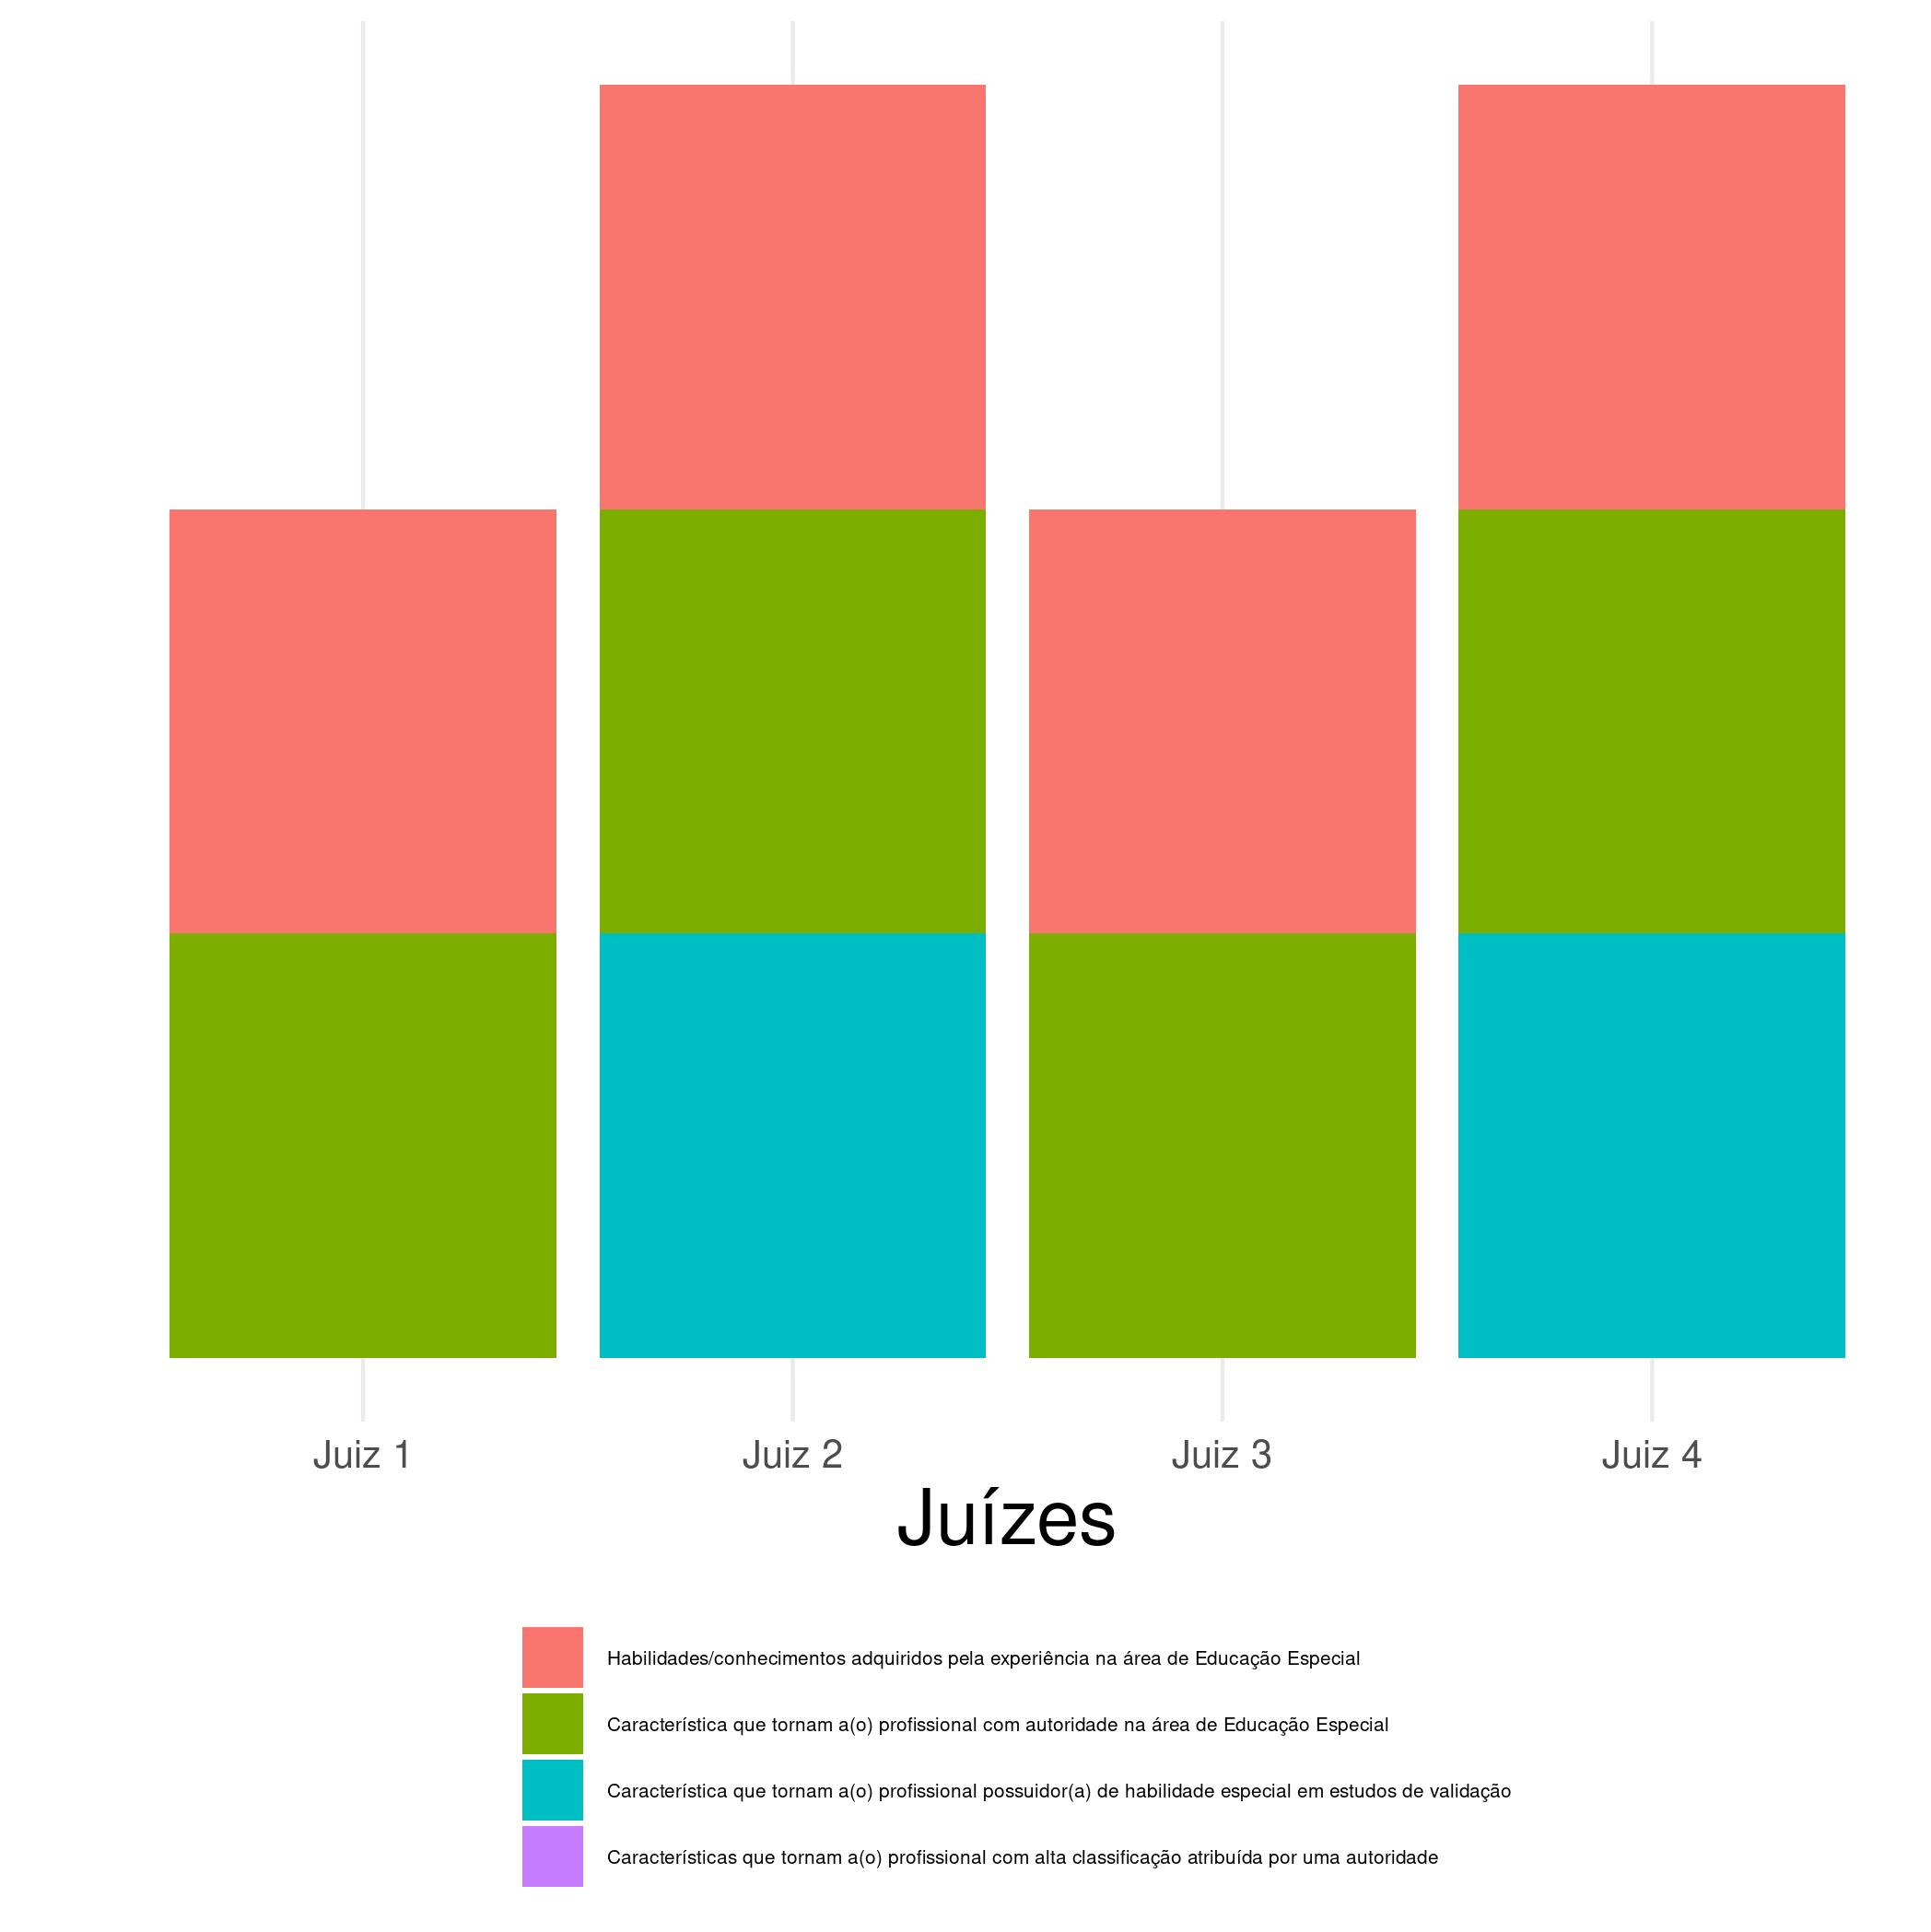
\includegraphics[width=0.9\linewidth]{figures/grafico1} 

}

\caption{Gráfico de distribuição das características dos juízes.}\label{fig:grafico1}
\end{figure}

\newpage

\hypertarget{gruxe1fico-do-coeficiente-de-validade-de-conteuxfado-em-relauxe7uxe3o-uxe0-clarezacompreensuxe3o-e-relevuxe2ncia-dos-itens-primeira-versuxe3o}{%
\subsection{Gráfico do Coeficiente de Validade de Conteúdo em relação à clareza/compreensão e relevância dos itens (primeira versão)}\label{gruxe1fico-do-coeficiente-de-validade-de-conteuxfado-em-relauxe7uxe3o-uxe0-clarezacompreensuxe3o-e-relevuxe2ncia-dos-itens-primeira-versuxe3o}}

Na Figura \ref{fig:grafico2V1}, incluimos o gráfico com o coeficiente CVC de clareza/compreensão e com o coeficiente de CVC de relevância para cada item. Além disso, incluímos o valor de referência recomendando por \protect\hyperlink{ref-hernandez2002contributions}{Hernández-Nieto} (\protect\hyperlink{ref-hernandez2002contributions}{2002}) que é \(0,8\). Como a amostra tem quatro juízes, o valor máximo do coeficiente CVC é \(1-\frac{1}{4}=0,75\) para esta amostra, abaixo do valor recomendado por \protect\hyperlink{ref-hernandez2002contributions}{Hernández-Nieto} (\protect\hyperlink{ref-hernandez2002contributions}{2002}), e, por isso, a linha azul que representa o \emph{valor mínimo de \(CVC_i\) para um item ter conteúdo válido} está acima de todas as barras na Figura \ref{fig:grafico2V1}.

\begin{figure}[htbp]

{\centering 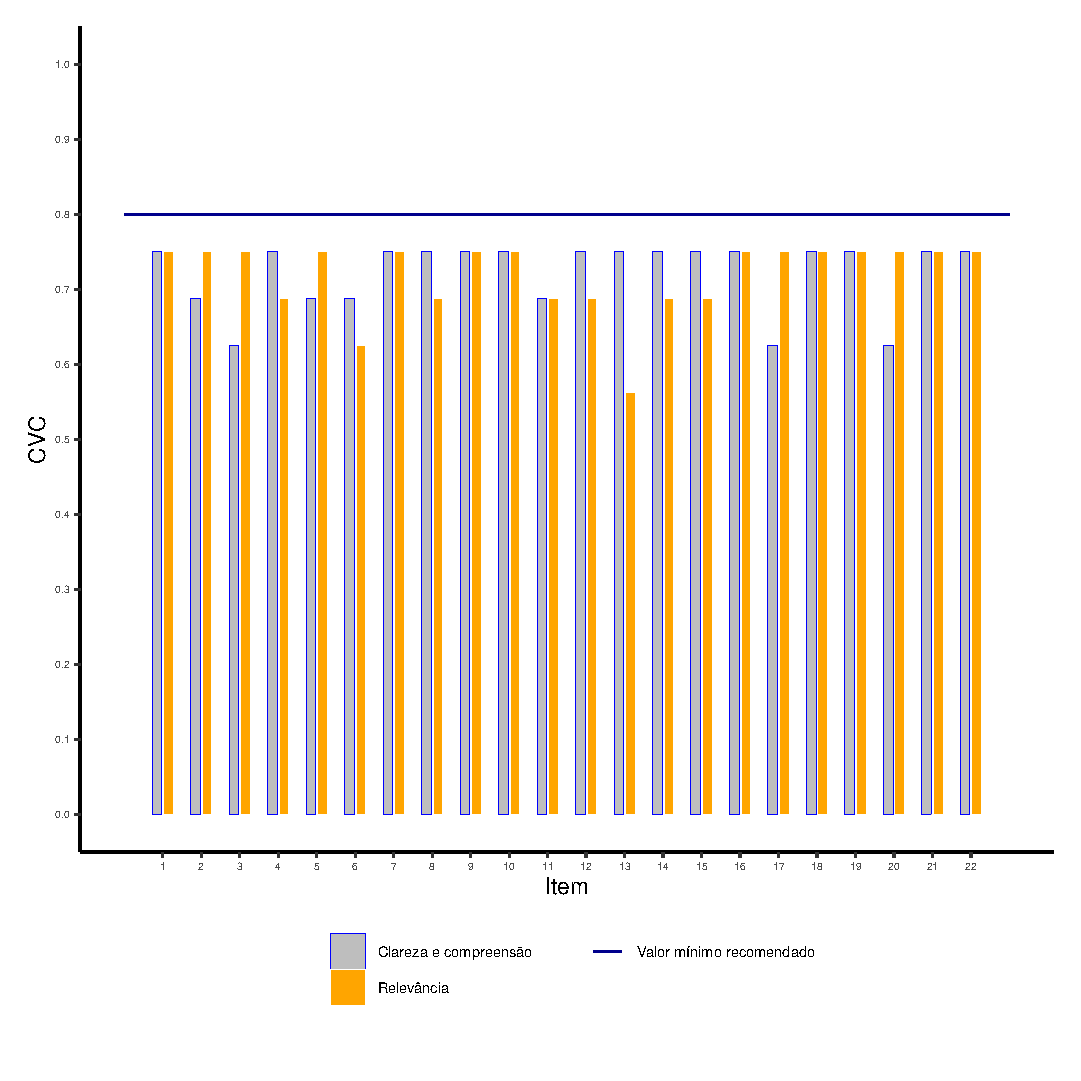
\includegraphics[width=0.9\linewidth]{figures/grafico2_0_8} 

}

\caption{Gráfico de distribuição das características dos juízes.}\label{fig:grafico2V1}
\end{figure}

\newpage

\hypertarget{gruxe1fico-do-coeficiente-de-validade-de-conteuxfado-em-relauxe7uxe3o-uxe0-clarezacompreensuxe3o-e-relevuxe2ncia-dos-itens-segunda-versuxe3o}{%
\subsection{Gráfico do Coeficiente de Validade de Conteúdo em relação à clareza/compreensão e relevância dos itens (segunda versão)}\label{gruxe1fico-do-coeficiente-de-validade-de-conteuxfado-em-relauxe7uxe3o-uxe0-clarezacompreensuxe3o-e-relevuxe2ncia-dos-itens-segunda-versuxe3o}}

Na Figura \ref{fig:grafico2V2}, incluimos o gráfico com o coeficiente CVC de clareza/compreensão e com o coeficiente de CVC de relevância para cada item. Além disso, incluímos o valor de referência \(0,6\). Como a amostra tem quatro juízes, o valor máximo do coeficiente CVC é \(1-\frac{1}{4}=0,75\) para esta amostra de juízes, e o consulente poderia usar \(80\%\) do valor máximo \(0,75\) que é \(0,6\).

\begin{figure}[htbp]

{\centering 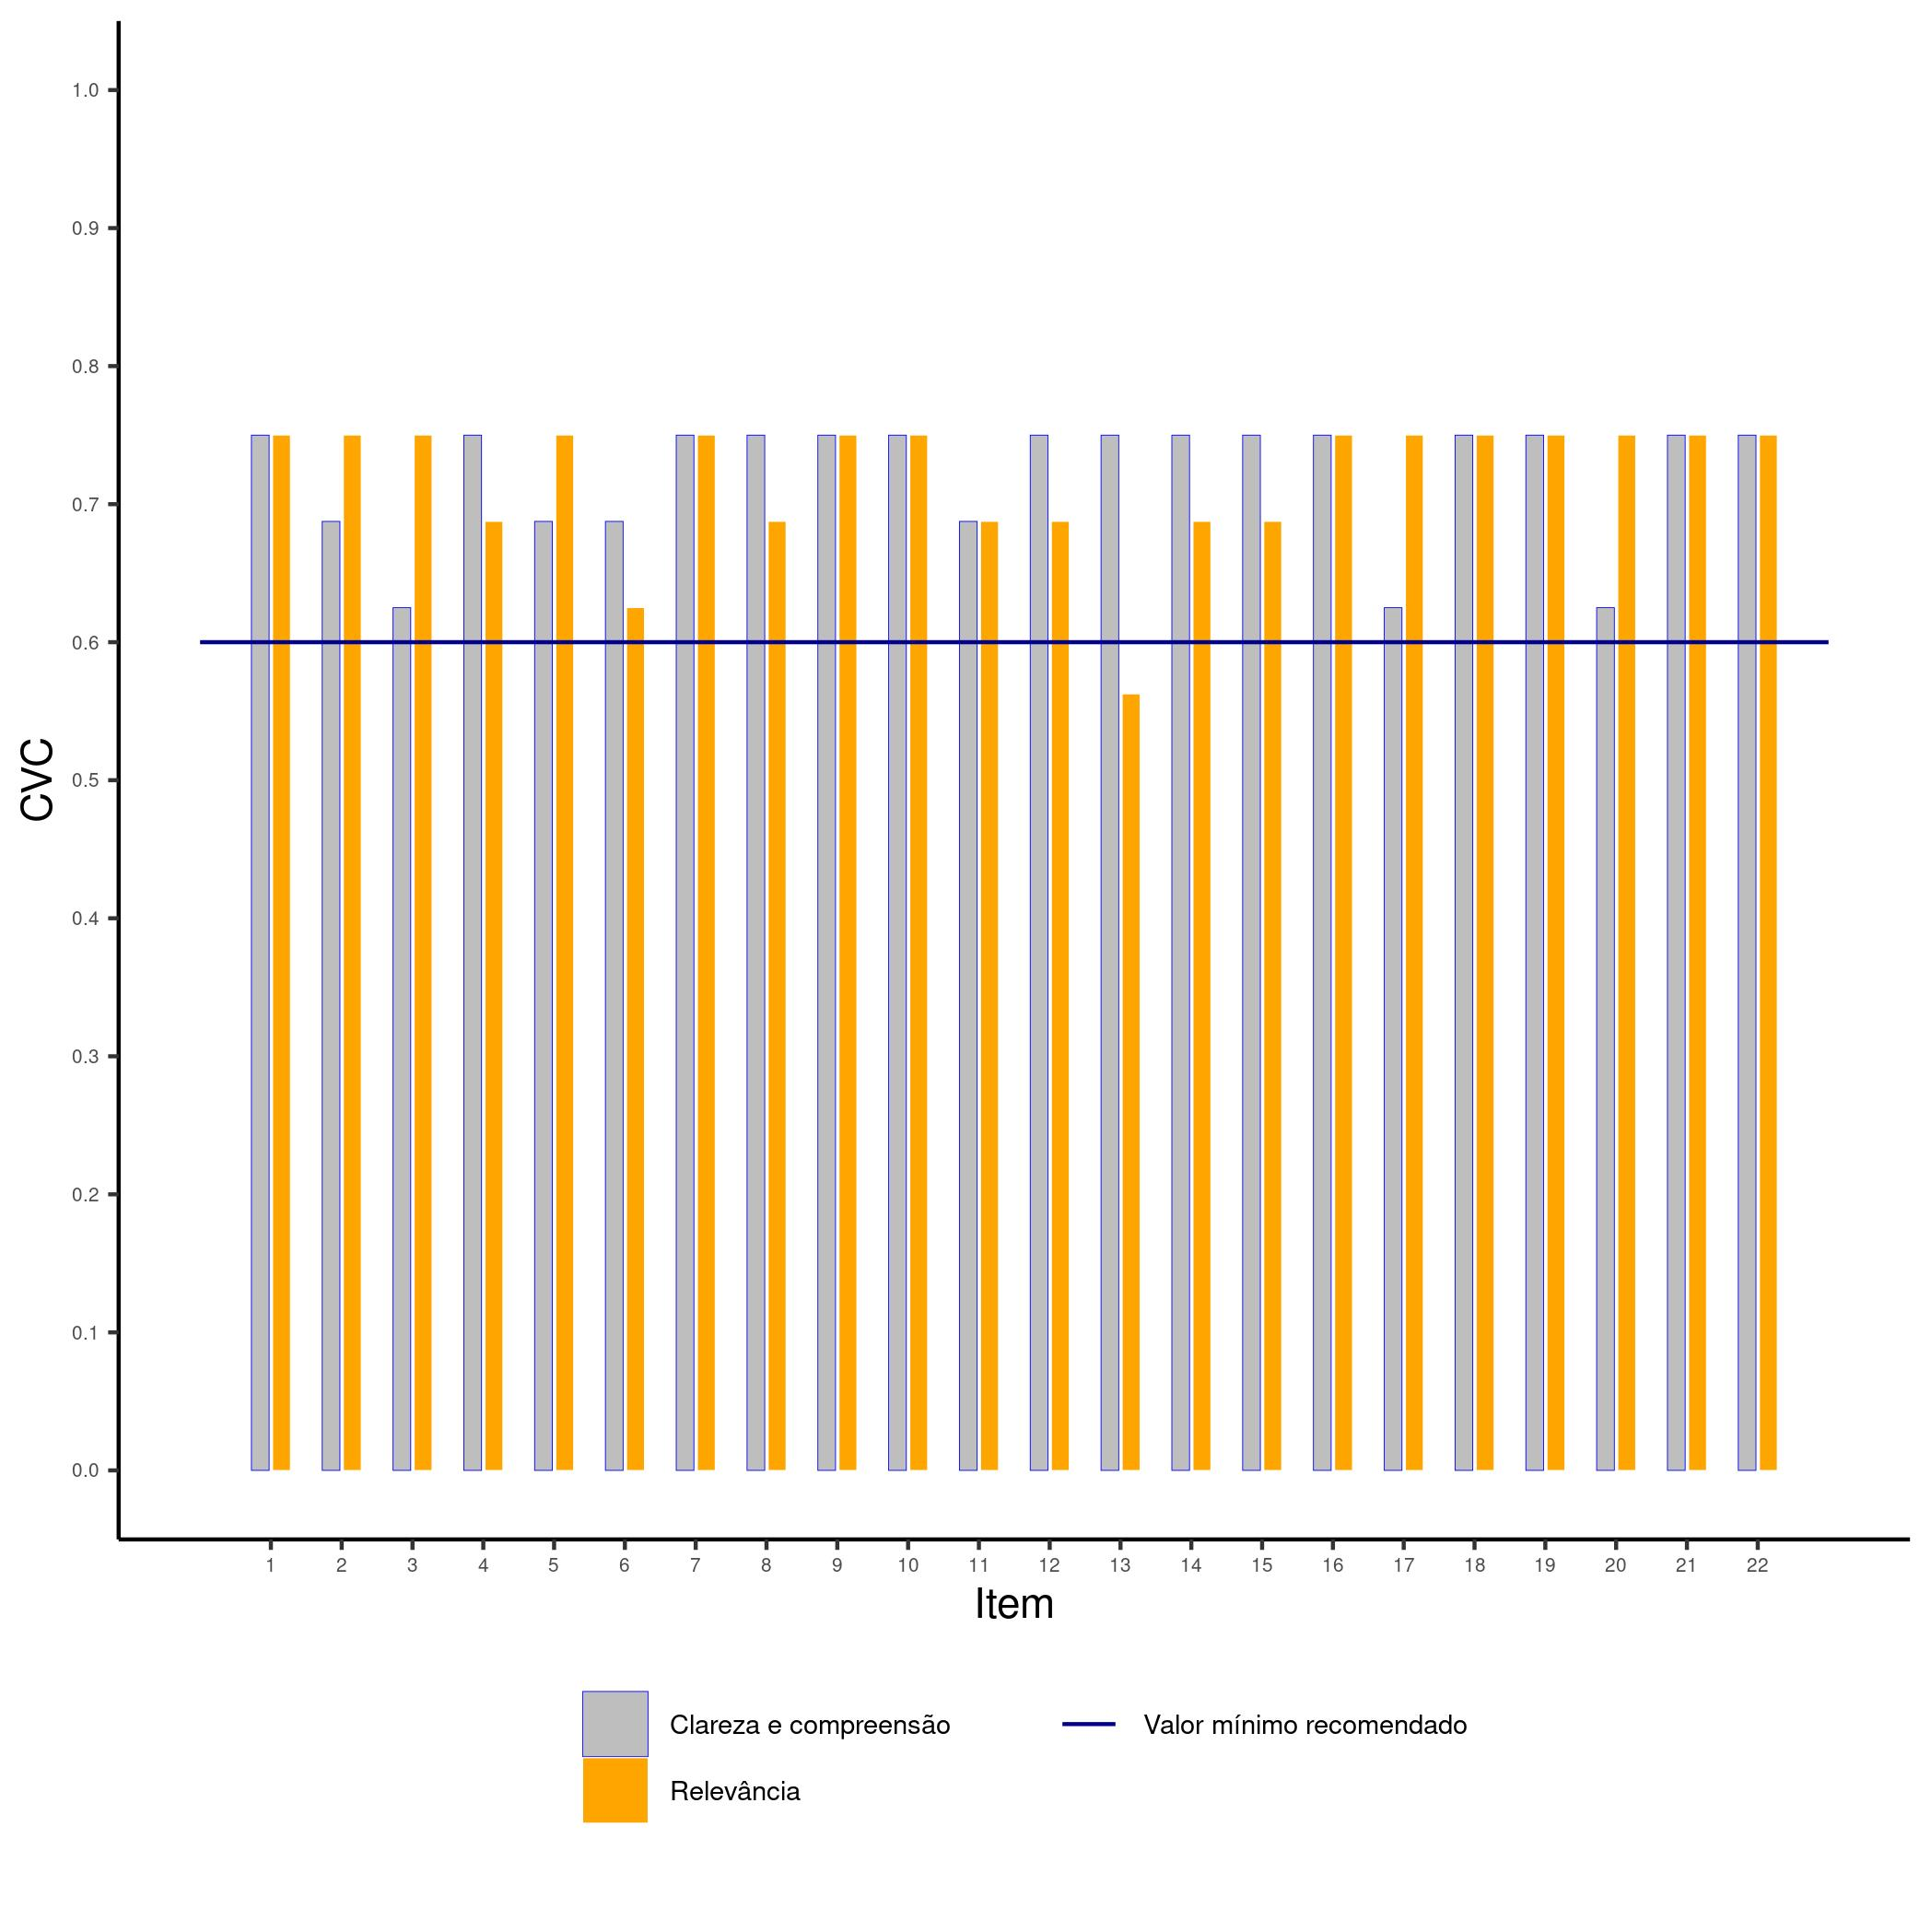
\includegraphics[width=0.9\linewidth]{figures/grafico2_80_perc} 

}

\caption{Gráfico de distribuição das características dos juízes.}\label{fig:grafico2V2}
\end{figure}

\newpage

\hypertarget{gruxe1fico-de-distribuiuxe7uxe3o-de-concorduxe2ncia-entre-os-juuxedzes}{%
\subsection{Gráfico de distribuição de concordância entre os juízes}\label{gruxe1fico-de-distribuiuxe7uxe3o-de-concorduxe2ncia-entre-os-juuxedzes}}

Na Figura \ref{fig:grafico3}, mostramos o gráfico de concordância entre os juízes sobre os construtos (Conhecimento, Atitude e Prática) de cada item. Os juízes apresentam uma alta concordância sobre os construtos (Conhecimento, Atitude e Prática) avaliados em cada item.

Para construir este gráfico, chequei se a resposta sobre o construto do item do juiz é igual ao construto do item pensado pelo consulente, e assumi que

\begin{enumerate}
\def\labelenumi{\arabic{enumi}.}
\tightlist
\item
  Questões 1 a 10 estão relacionadas ao construto \emph{Conhecimento} (segundo o consulente);
\item
  Questões 11 a 17 estão relacionadas ao construto \emph{Atitude} (segundo o consulente);
\item
  Questões 18 a 22 estão relacionadas ao construto \emph{Prática} (segundo o consulente).
\end{enumerate}

O consulente não forneceu essas informações, e eu as inferi. Sugiro que o consulente confira e confirme estas informações.

\begin{figure}[htbp]

{\centering 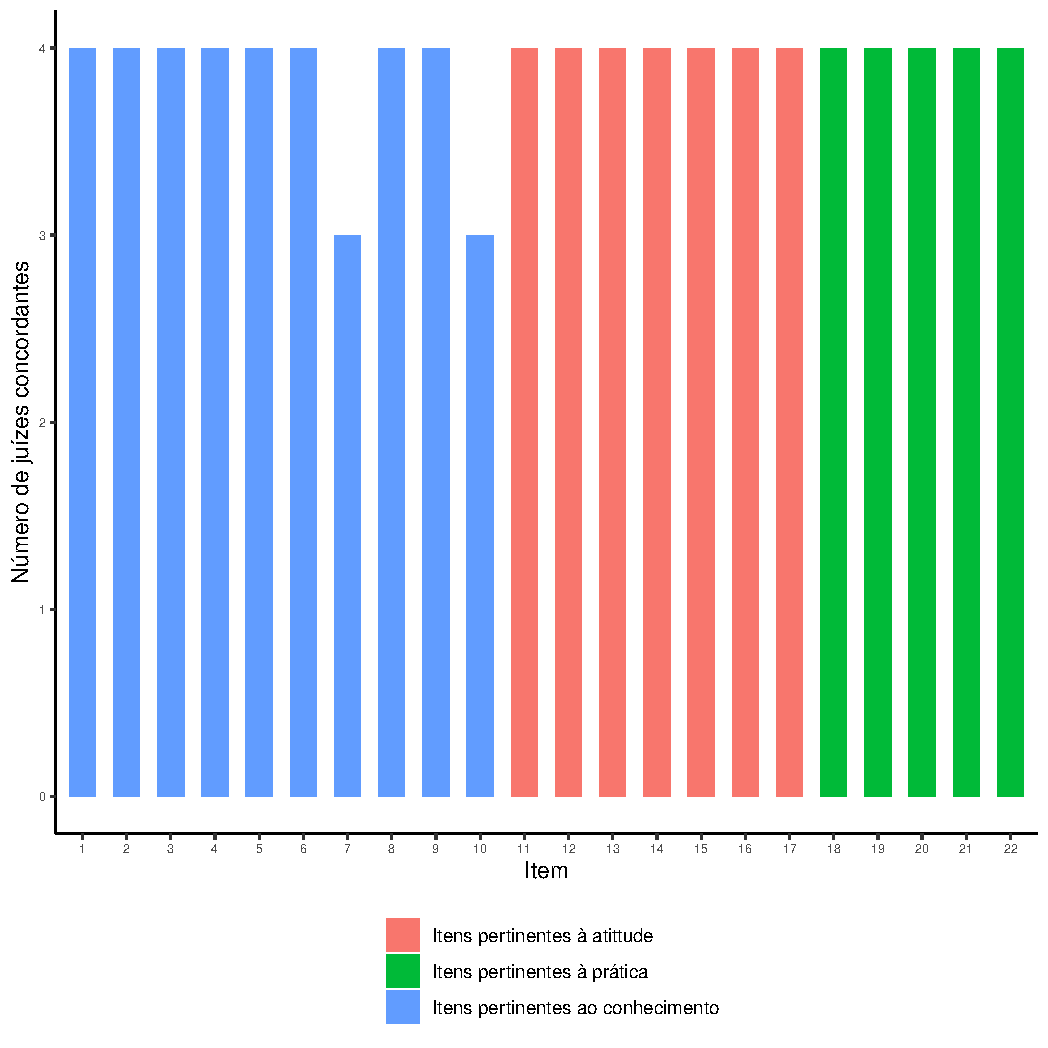
\includegraphics[width=0.75\linewidth]{figures/grafico3} 

}

\caption{Número de juízes concordantes.}\label{fig:grafico3}
\end{figure}

\newpage

\hypertarget{tabela-do-perfil-dos-especialistas-segundos-os-atributos}{%
\subsection{Tabela do perfil dos especialistas segundos os atributos}\label{tabela-do-perfil-dos-especialistas-segundos-os-atributos}}

Na Tabela \ref{tab:atributo}, mostramos que as características dos juízes selecionados se distribuem de forma representativa nos atributos, com exceção ao atributo \emph{homenagem/menção honrosa de reconhecimento como autoridade na área de Educação Especial e/ou Transtorno do Espectro Autista, recebida de instituição científica}.

\begin{table}[htbp]
\caption{Atributo / característica profissional.}
\label{tab:atributo}
\scalebox{0.65}{
\begin{tabular}{|l|r|}
\hline
\textbf{Habilidades/conhecimentos adquirido pela experiência na área de Educação Especial} & \multicolumn{1}{l|}{\textbf{}} \\ \hline
Tempo mínimo de 5 anos de experiência profissional assistencial na área de Educação Especial & 4 \\ \hline
Tempo mínimo de 5 anos de experiência docente na área de Educação Especial & 0 \\ \hline
\textbf{Característica que tornam a (o) profissional autoridade  na área de Educação Especial} & \multicolumn{1}{l|}{\textbf{}} \\ \hline
Convidado em evento científico nacional ou internacional na área de Educação Especial e/ou
Transtorno do Espectro Autista como palestrante & 3 \\ \hline
Orientou trabalhos acadêmicos de Pós-graduação Stricto sensu com temática relativa à área de
 Educação Especial e/ou Transtorno do Espectro Autista? & 3 \\ \hline
Autoria em artigos (s) científicos na área de Educação Especial e/ou Transtorno do Espectro Autista & 4 \\ \hline
Pós-graduação Stricto sensu com dissertação ou tese em temática relativa na área de
 Educação Especial e/ou Transtorno do Espectro Autista & 4 \\ \hline
Participação em banca(s) avaliadora(s) de trabalhos acadêmico de Pós-graduação Stricto Sensu
 com temática relativa na área de Educação Especial e/ou Transtorno do Espectro Autista & 2 \\ \hline
\textbf{Característica que tornam o profissional possuidor de habilidade especial em estudos de validação } & \multicolumn{1}{l|}{\textbf{}} \\ \hline
Orientou trabalhos de Pós-graduação Stricto sensu com temática relativa
 à validação de instrumentos de coleta de dados  & 2 \\ \hline
Autoria em artigo (s) científicos na área de validação de instrumento de coleta de dados  & 1 \\ \hline
Pós-graduação Stricto sensu com pesquisa na área de validação de instrumentos  & 2 \\ \hline
Participação em banca(s) avaliadora(s) de trabalhos acadêmico de Pós-graduação Stricto Sensu
 com temática relativa na área de validação de instrumento de coleta de dados & 0 \\ \hline
\textbf{Características que tornam o profissional com alta classificação atribuída por uma autoridade } & \multicolumn{1}{l|}{\textbf{}} \\ \hline
Homenagem/menção honrosa de reconhecimento como autoridade na área
 de Educação Especial e/ou Transtorno do Espectro Autista, recebida de instituição científica & 0 \\ \hline
Trabalhos premiados em eventos científicos nacionais e internacionais cujo conteúdo
 seja referente à área de uroginecologia  & 0 \\ \hline
Trabalhos premiados em eventos científicos nacionais e internacionais cujo
 conteúdo seja referente à área de validação de instrumento de coleta de dados  & 0 \\ \hline
\textbf{Total de juízes } & \textbf{10} \\ \hline
\end{tabular}
}
\end{table}

\newpage

\hypertarget{tabela-com-o-coeficiente-kappa-de-cohen-para-cada-par-de-juuxedzes}{%
\subsection{Tabela com o coeficiente Kappa de Cohen para cada par de juízes}\label{tabela-com-o-coeficiente-kappa-de-cohen-para-cada-par-de-juuxedzes}}

Na Tabela \ref{tab:kappa}, calculamos o coeficiente Kappa para cada par de juízes, onde incluimos o valor do Coeficiente Kappa como descrito por \protect\hyperlink{ref-firmiano2017escala}{Firmiano} (\protect\hyperlink{ref-firmiano2017escala}{2017}), incluimos também o Intervalo de Confiança (IC) com coeficiente de confiança \(\gamma=95\%\) para cada par de de juízes e o valor-p para o teste de hipóteses com a hipótese nula dada por \(H_0: \kappa = 0\) e hipótese alternativa dada por \(H_1: \kappa > 0\) (valores pequenos do valor-p indicam que devemos rejeitar de \(H_0\) em favor de \(H_1\)).

Além disso, o cálculo de Coeficiente Kappa para todo o instrumento é \(0,9296\) com valor-p aproximadamente zero (e rejeitamos \(H_0: \kappa = 0\) e em favor de \(H_1: \kappa >0\)).

\begin{table}[htbp]
\centering
\caption{Cálculo do Coeficiente Kappa de Concordância entre dois juízes.}
\scalebox{0.75}{
\begin{tabular}{cc|ccccc}
\toprule
Primeiro juiz & Segundo juiz & Coeficiente Kappa ($\kappa$) & Limite inferior IC & Limite superior IC & Coeficiente de confiança & valor-p \\ \midrule
Juiz 1 & Juiz 2 & 0,8599 & 0,6747 & 1,0000 & 0,95 & 0,0000 \\ 
Juiz 1 & Juiz 3 & 0,9297 & 0,7951 & 1,0000 & 0,95 & 0,0000 \\ 
Juiz 1 & Juiz 4 & 0,9297 & 0,7951 & 1,0000 & 0,95 & 0,0000 \\ 
Juiz 2 & Juiz 3 & 0,9297 & 0,7951 & 1,0000 & 0,95 & 0,0000 \\ 
Juiz 2 & Juiz 4 & 0,9297 & 0,7951 & 1,0000 & 0,95 & 0,0000 \\ 
Juiz 3 & Juiz 4 & 1,0000 & 1,0000 & 1,0000 & 0,95 & 0,0000 \\ \bottomrule
\end{tabular}
}
\label{tab:kappa}
\end{table}

Usamos a seguinte codificação para os juízes:

\begin{itemize}
\tightlist
\item
  \textbf{Juiz 1} corresponde ao juiz com endereço de e-mail dado por \href{mailto:monica_scattolin@yahoo.com.br}{\nolinkurl{monica\_scattolin@yahoo.com.br}};
\item
  \textbf{Juiz 2} corresponde ao juiz com endereço de e-mail dado por \href{mailto:paolaokuda@yahoo.com.br}{\nolinkurl{paolaokuda@yahoo.com.br}};
\item
  \textbf{Juiz 3} corresponde ao juiz com endereço de e-mail dado por \href{mailto:biaamoraes@gmail.com}{\nolinkurl{biaamoraes@gmail.com}};
\item
  \textbf{Juiz 4} corresponde ao juiz com endereço de e-mail dado por \href{mailto:lucelmolacerda@gmail.com}{\nolinkurl{lucelmolacerda@gmail.com}}.
\end{itemize}

\cleardoublepage

\hypertarget{referuxeancias}{%
\section*{Referências}\label{referuxeancias}}
\addcontentsline{toc}{section}{Referências}

\hypertarget{refs}{}
\begin{CSLReferences}{1}{0}
\leavevmode\hypertarget{ref-firmiano2017escala}{}%
Firmiano, Maria Luisa Veras. 2017. {``Escala de Avaliação Do Conhecimento, Atitude e Prática de Gestantes Sobre Incontinência Urinária: Construção e Validação de Conteúdo.''} Master's thesis, Universidade Federal do Ceará.

\leavevmode\hypertarget{ref-fleiss1981measurement}{}%
Fleiss, Joseph L, Bruce Levin, Myunghee Cho Paik, and others. 1981. {``The Measurement of Interrater Agreement.''} \emph{Statistical Methods for Rates and Proportions} 2 (212-236): 22--23.

\leavevmode\hypertarget{ref-irr2019package}{}%
Gamer, Matthias, Jim Lemon, and Ian Fellows Puspendra Singh. 2019. \emph{Irr: Various Coefficients of Interrater Reliability and Agreement}. \url{https://CRAN.R-project.org/package=irr}.

\leavevmode\hypertarget{ref-hernandez2002contributions}{}%
Hernández-Nieto, Rafael A. 2002. {``Contributions to Statistical Analysis.''} \emph{M{é}rida: Universidad de Los Andes} 193.

\leavevmode\hypertarget{ref-jasper1994expert}{}%
Jasper, Melanie A. 1994. {``Expert: A Discussion of the Implications of the Concept as Used in Nursing.''} \emph{Journal of Advanced Nursing} 20 (4): 769--76.

\leavevmode\hypertarget{ref-kraemer2014kappa}{}%
Kraemer, Helena C. 2014. {``Kappa Coefficient.''} \emph{Wiley StatsRef: Statistics Reference Online}, 1--4.

\leavevmode\hypertarget{ref-fmsb2021package}{}%
Nakazawa, Minato. 2021. \emph{Fmsb: Functions for Medical Statistics Book with Some Demographic Data}. \url{https://CRAN.R-project.org/package=fmsb}.

\leavevmode\hypertarget{ref-pasquali1999elaboraccao}{}%
Pasquali, L. 1999. \emph{Elaboração de Instrumentos Psicológicos: Manual Prático de Elaboração}. LabPAM/IBAPP, Brasília, DF: IBAPP.

\leavevmode\hypertarget{ref-Rlang}{}%
R Core Team. 2021. \emph{R: A Language and Environment for Statistical Computing}. Vienna, Austria: R Foundation for Statistical Computing. \url{https://www.R-project.org/}.

\end{CSLReferences}

\end{document}
